%\begin{enumerate}[label=\thesubsection.\arabic*.,ref=\thesubsection.\theenumi]
%\numberwithin{equation}{enumi}

% 
Consider the system shown in Fig. \ref{fig:ee18btech11034}
below. Sketch the nyquist plot of the system when
\begin{enumerate}
\item $G_c(s) = 1$
\item $G_c(s) = 1+\frac{1}{s}$
\end{enumerate} 

and determine the maximum value of $K$ for stability.
Take  
\begin{align}
G\brak{s} = \frac{K}{s\brak{1+s}\brak{1+4s}}
\label{eq:ee18btech11034_Gs}
\end{align}

\begin{figure}[!ht]
	\begin{center}
		
		\resizebox{\columnwidth}{!}{\input{./figs/ee18btech11034/ee18btech11034_fig.tex}}
	\end{center}
\caption{}
\label{fig:ee18btech11034}
\end{figure}

\solution
 For $G_{c}\brak{s}$ = 1,

The open loop transfer function is 
\begin{align}
    G_{c}\brak{s}G\brak{s} = \frac{K}{s\brak{1+s}\brak{1+4s}}
\end{align}

\begin{align}
    G_{c}\brak{\j\omega}G\brak{\j\omega} &= \frac{K}{{\j\omega}\brak{1+\j\omega}\brak{1+4\j\omega}}
    \\
    &= \frac{K}{{\j\omega}\brak{1-4\omega^2+5\j\omega}}
    \\
    &= \frac{K\brak{-5\omega-\j\brak{1-4\omega^2}}}{{\omega}\brak{\brak{1-4\omega^2}^2+25\omega^2}}
    \end{align}
The maximum K for stability is where the nyquist plot of open loop transfer function cuts the coordinate \brak{-1,\j0}


\begin{align}
 \implies    \text{Re} \cbrak{G\brak{\j \omega}G_{c}\brak{\j\omega}} &= -1
 \label{eq:ee18btech11034_eq_Re}
 \\
 \implies \text{Im} \cbrak{G\brak{\j \omega}G_{c}\brak{\j\omega}} &= 0
 \label{eq:ee18btech11034_eq_Im}
\end{align}

\begin{align}
 \implies    \text{Re} \cbrak{G\brak{\j \omega}G_{c}\brak{\j\omega}} &= \frac{-5K\omega}{{\omega}\brak{\brak{1-4\omega^2}^2+25\omega^2}}
 \label{eq:ee18btech11034_eq_1_Re}
 \\
 \implies \text{Im} \cbrak{G\brak{\j \omega}G_{c}\brak{\j\omega}} &= \frac{-K\brak{1-4\omega^2}}{{\omega}\brak{\brak{1-4\omega^2}^2+25\omega^2}}
 \label{eq:ee18btech11034_eq_1_Im}
\end{align}

From \eqref{eq:ee18btech11034_eq_1_Im} and \eqref{eq:ee18btech11034_eq_Im}
\begin{align}
    1-4\omega^2 = 0
    \implies \omega = \frac{1}{2} 
\end{align}
From  \eqref{eq:ee18btech11034_eq_1_Re},\eqref{eq:ee18btech11034_eq_Re} and substituting $\omega = \frac{1}{2}$
\begin{align}
    \frac{-5K\brak{\frac{1}{2}}}{\brak{\frac{1}{2}}\brak{\frac{25}{4}}} = -1
    \implies K = \frac{5}{4} = 1.25
\end{align}

For $K < 0$ the system with negative feedback is unstable the range of K is 
\begin{align}
    0 < K < \frac{5}{4}
\end{align}
 Sketching the Nyquist plot for $G(s)G_c(s)$ in Fig. \ref{fig:ee18btech11034_1}
The following code gives the nyquist plot
\begin{lstlisting}
codes/ee18btech11034/ee18btech11034_1.py
\end{lstlisting}

\begin{figure}[!h]
\centering
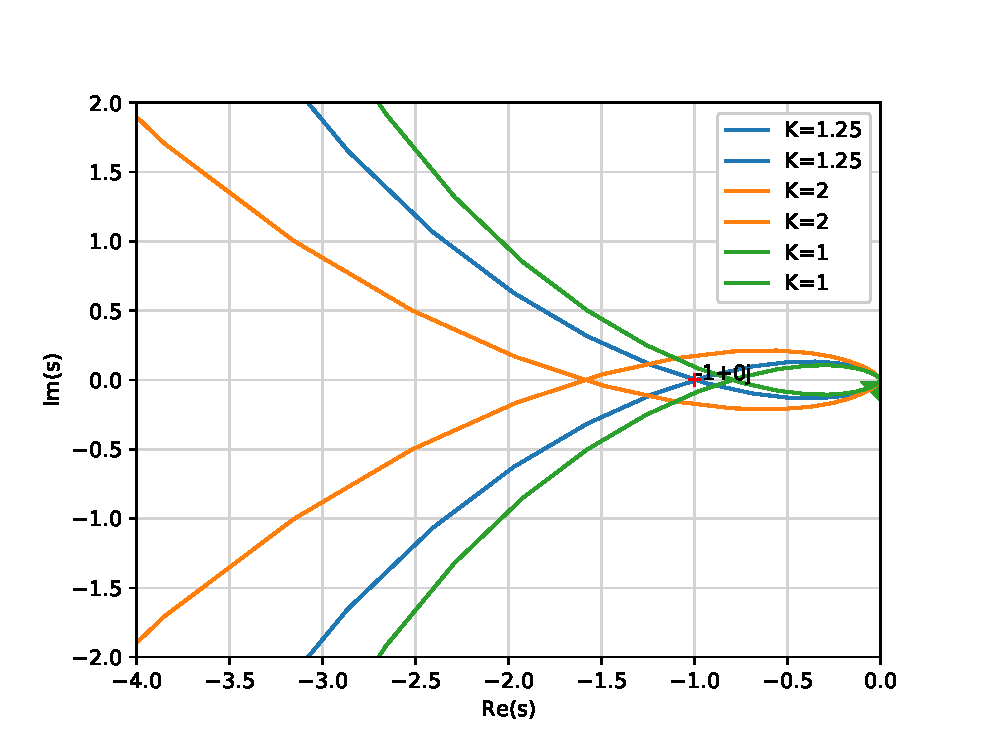
\includegraphics[width=\columnwidth]{./figs/ee18btech11034/ee18btech11034_1.eps}
\caption{}
\label{fig:ee18btech11034_1}
\end{figure}
 Stability Criterian for K
\begin{align}
    N + P = Z
    \label{eq:ee18btech11034_Z}
\end{align}
\begin{table}[!ht]
\centering
\input{./tables/ee18btech11034/ee18btech11034_table1.tex}
\caption{}
\label{table:ee18btech11034_table1}
\end{table}

From the Fig.\ref{fig:ee18btech11034_1}  
\begin{align}
 K_{max} = \frac{5}{4}  
\end{align}


\solution
For $G_{c}\brak{s} = \frac{1+s}{s}$,

the open loop transfer function is 
\begin{align}
    G_{c}\brak{s}G\brak{s} &= \frac{K\brak{s+1}}{s^2\brak{1+s}\brak{1+4s}}
\end{align}
\begin{align}
    G_{c}\brak{s}G\brak{s} &= \frac{K}{s^2\brak{1+4s}}
\end{align}
\begin{align}
    G_{c}\brak{\j\omega}G\brak{\j\omega} &= \frac{K}{\brak{\j\omega}^2\brak{1+4\j\omega}}
    \\
    &= \frac{\frac{-K}{\omega^2}\brak{1-4\j\omega}}{1+16\omega^2}
\end{align}
From \eqref{eq:ee18btech11034_eq_Im}
\begin{align}
    \implies \text{Im} \cbrak{G\brak{\j \omega}G_{c}\brak{\j\omega}} &= \frac{4K}{{\omega}\brak{1+16\omega^2}} &= 0
\end{align}
This is possible when 
\begin{align}
    K = 0
    \label{eq:ee18btech11034_3}
\end{align}

The system is unstable for both 
\begin{align}
    K &< 0
\end{align}
\begin{align}
    K &> 0
\end{align}

 Sketching the Nyquist plot for $G(s)G_c(s)$ in Fig. \ref{fig:ee18btech11034_2}
The following code gives the nyquist plot
\begin{lstlisting}
codes/ee18btech11034/ee18btech11034_2.py
\end{lstlisting}
\begin{figure}[!h]
\centering
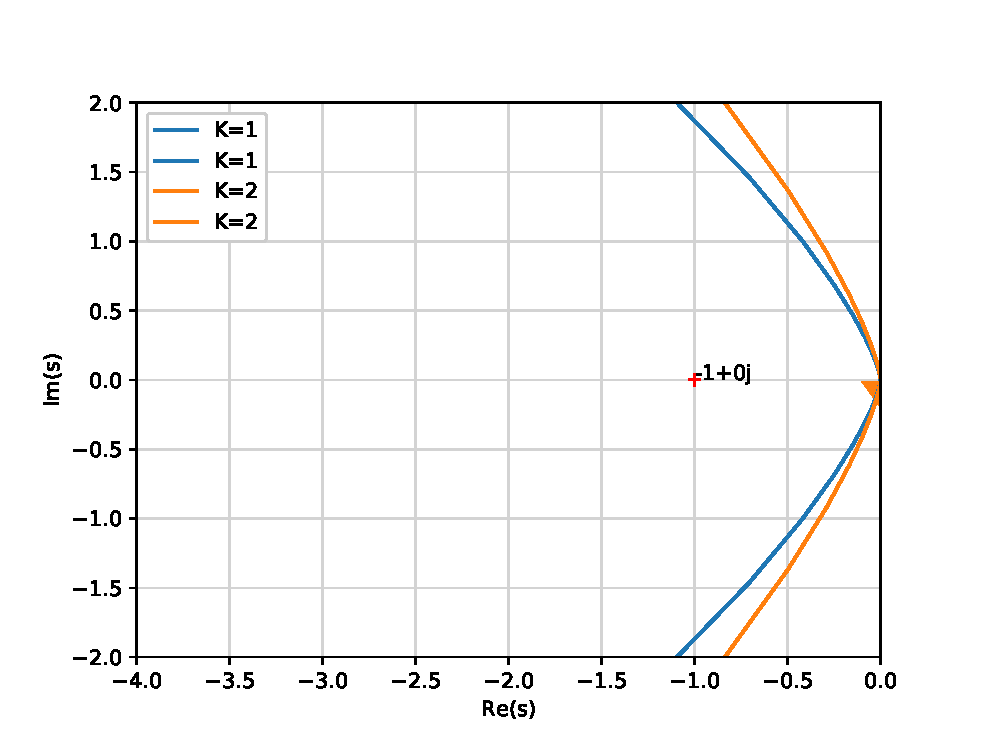
\includegraphics[width=\columnwidth]{./figs/ee18btech11034/ee18btech11034_2.eps}
\caption{}
\label{fig:ee18btech11034_2}
\end{figure}
From \eqref{eq:ee18btech11034_Z}

\begin{table}[!ht]
\centering
\input{./tables/ee18btech11034/ee18btech11034_table2.tex}
\caption{}
\label{table:ee18btech11034_table2}
\end{table}
From \eqref{eq:ee18btech11034_3} $K_{max}$ must be 0 which is not possible.
Hence the system is unstable for all real K
%\end{enumerate}
